\chapter{Razapinjuća stabla}

\index{razapinjuće stablo}

\key{Razapinjuće stablo} grafa sastoji se od
svih čvorova grafa i nekih od
bridova grafa tako da postoji put
između svaka dva čvora.
Kao i stabla općenito, razapinjuća stabla su
povezana i aciklična.
Obično postoji više načina da konstruiramo razapinjuće stablo.

Na primjer, razmotrimo sljedeći graf:
\begin{center}
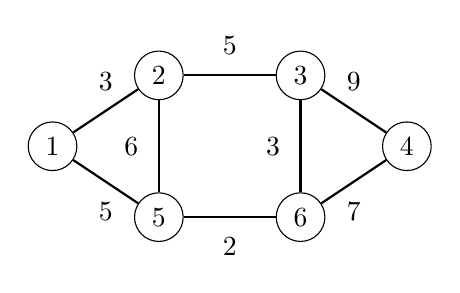
\begin{tikzpicture}[scale=0.9]
\node[draw, circle] (1) at (1.5,2) {$1$};
\node[draw, circle] (2) at (3,3) {$2$};
\node[draw, circle] (3) at (5,3) {$3$};
\node[draw, circle] (4) at (6.5,2) {$4$};
\node[draw, circle] (5) at (3,1) {$5$};
\node[draw, circle] (6) at (5,1) {$6$};
\path[draw,thick,-] (1) -- node[font=\small,label=above:3] {} (2);
\path[draw,thick,-] (2) -- node[font=\small,label=above:5] {} (3);
\path[draw,thick,-] (3) -- node[font=\small,label=above:9] {} (4);
\path[draw,thick,-] (1) -- node[font=\small,label=below:5] {} (5);
\path[draw,thick,-] (5) -- node[font=\small,label=below:2] {} (6);
\path[draw,thick,-] (6) -- node[font=\small,label=below:7] {} (4);
\path[draw,thick,-] (2) -- node[font=\small,label=left:6] {} (5);
\path[draw,thick,-] (3) -- node[font=\small,label=left:3] {} (6);
\end{tikzpicture}
\end{center}
Jedno razapinjuće stablo tog grafa je sljedeće:
\begin{center}
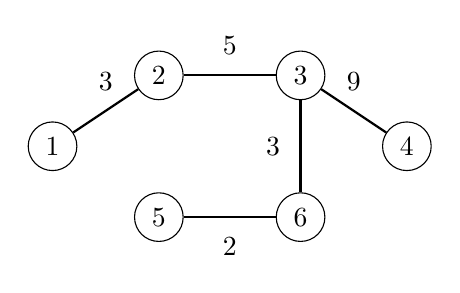
\begin{tikzpicture}[scale=0.9]
\node[draw, circle] (1) at (1.5,2) {$1$};
\node[draw, circle] (2) at (3,3) {$2$};
\node[draw, circle] (3) at (5,3) {$3$};
\node[draw, circle] (4) at (6.5,2) {$4$};
\node[draw, circle] (5) at (3,1) {$5$};
\node[draw, circle] (6) at (5,1) {$6$};
\path[draw,thick,-] (1) -- node[font=\small,label=above:3] {} (2);
\path[draw,thick,-] (2) -- node[font=\small,label=above:5] {} (3);
\path[draw,thick,-] (3) -- node[font=\small,label=above:9] {} (4);
\path[draw,thick,-] (5) -- node[font=\small,label=below:2] {} (6);
\path[draw,thick,-] (3) -- node[font=\small,label=left:3] {} (6);
\end{tikzpicture}
\end{center}

Težina razapinjućeg stabla je suma težina njegovih bridova.
Na primjer, težina gornjeg razapinjućeg stabla iznosi
$3+5+9+3+2=22$.

\index{minimalno razapinjuće stablo}

\key{Minimalno razapinjuće stablo}
je razapinjuće stablo čija je težina najmanja moguća.
Težina minimalnog razapinjućeg stabla za graf iz primjera
iznosi 20, a takvo stablo možemo konstruirati na sljedeći način:

\begin{center}
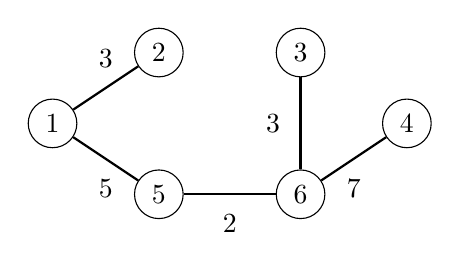
\begin{tikzpicture}[scale=0.9]
\node[draw, circle] (1) at (1.5,2) {$1$};
\node[draw, circle] (2) at (3,3) {$2$};
\node[draw, circle] (3) at (5,3) {$3$};
\node[draw, circle] (4) at (6.5,2) {$4$};
\node[draw, circle] (5) at (3,1) {$5$};
\node[draw, circle] (6) at (5,1) {$6$};

\path[draw,thick,-] (1) -- node[font=\small,label=above:3] {} (2);
\path[draw,thick,-] (1) -- node[font=\small,label=below:5] {} (5);
\path[draw,thick,-] (5) -- node[font=\small,label=below:2] {} (6);
\path[draw,thick,-] (6) -- node[font=\small,label=below:7] {} (4);
\path[draw,thick,-] (3) -- node[font=\small,label=left:3] {} (6);
\end{tikzpicture}
\end{center}

\index{maksimalno razapinjuće stablo}

Na sličan način, \key{maksimalno razapinjuće stablo}
je razapinjuće stablo čija je težina najveća moguća.
Težina maksimalnog razapinjućeg stabla za
graf iz primjera iznosi 32:

\begin{center}
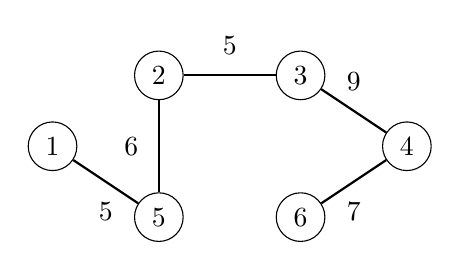
\begin{tikzpicture}[scale=0.9]
\node[draw, circle] (1) at (1.5,2) {$1$};
\node[draw, circle] (2) at (3,3) {$2$};
\node[draw, circle] (3) at (5,3) {$3$};
\node[draw, circle] (4) at (6.5,2) {$4$};
\node[draw, circle] (5) at (3,1) {$5$};
\node[draw, circle] (6) at (5,1) {$6$};
\path[draw,thick,-] (2) -- node[font=\small,label=above:5] {} (3);
\path[draw,thick,-] (3) -- node[font=\small,label=above:9] {} (4);
\path[draw,thick,-] (1) -- node[font=\small,label=below:5] {} (5);
\path[draw,thick,-] (6) -- node[font=\small,label=below:7] {} (4);
\path[draw,thick,-] (2) -- node[font=\small,label=left:6] {} (5);
\end{tikzpicture}
\end{center}

Uočimo da graf može imati više
minimalnih i maksimalnih razapinjućih stabala,
pa ta stabla nisu jedinstvena.

Pokazuje se da za konstrukciju minimalnih i maksimalnih
razapinjućih stabala možemo koristiti
više pohlepnih metoda.
U ovom poglavlju razmatramo dva algoritma
koji obrađuju
bridove grafa poredane po njihovim težinama.
Usredotočujemo se na traženje minimalnih razapinjućih stabala,
no isti algoritmi mogu naći
maksimalna razapinjuća stabla ako bridove obrađujemo u obrnutom redoslijedu.

\section{Kruskalov algoritam}

\index{Kruskalov algoritam}

U \key{Kruskalovom algoritmu}\footnote{Algoritam je 1956. godine
objavio J. B. Kruskal \cite{kru56}.} početno razapinjuće stablo
sadrži samo čvorove grafa
i ne sadrži nijedan brid.
Zatim algoritam prolazi kroz bridove
poredane po njihovim težinama i uvijek dodaje brid
u stablo ako on ne stvara ciklus.

Algoritam održava komponente
stabla.
Na početku svaki čvor grafa
pripada zasebnoj komponenti.
Svaki put kad se brid doda u stablo,
spajaju se dvije komponente.
Na kraju svi čvorovi pripadaju istoj komponenti
i minimalno razapinjuće stablo je nađeno.

\subsubsection{Primjer}

\begin{samepage}
Razmotrimo kako Kruskalov algoritam obrađuje
sljedeći graf:
\begin{center}
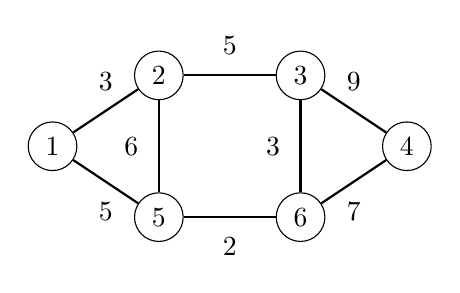
\begin{tikzpicture}[scale=0.9]
\node[draw, circle] (1) at (1.5,2) {$1$};
\node[draw, circle] (2) at (3,3) {$2$};
\node[draw, circle] (3) at (5,3) {$3$};
\node[draw, circle] (4) at (6.5,2) {$4$};
\node[draw, circle] (5) at (3,1) {$5$};
\node[draw, circle] (6) at (5,1) {$6$};
\path[draw,thick,-] (1) -- node[font=\small,label=above:3] {} (2);
\path[draw,thick,-] (2) -- node[font=\small,label=above:5] {} (3);
\path[draw,thick,-] (3) -- node[font=\small,label=above:9] {} (4);
\path[draw,thick,-] (1) -- node[font=\small,label=below:5] {} (5);
\path[draw,thick,-] (5) -- node[font=\small,label=below:2] {} (6);
\path[draw,thick,-] (6) -- node[font=\small,label=below:7] {} (4);
\path[draw,thick,-] (2) -- node[font=\small,label=left:6] {} (5);
\path[draw,thick,-] (3) -- node[font=\small,label=left:3] {} (6);
\end{tikzpicture}
\end{center}
\end{samepage}

\begin{samepage}
Prvi korak algoritma je sortiranje
bridova u rastućem redoslijedu njihovih težina.
Rezultat je sljedeća lista:

\begin{tabular}{ll}
\\
brid & težina \\
\hline
5--6 & 2 \\
1--2 & 3 \\
3--6 & 3 \\
1--5 & 5 \\
2--3 & 5 \\
2--5 & 6 \\
4--6 & 7 \\
3--4 & 9 \\
\\
\end{tabular}
\end{samepage}

Nakon toga algoritam prolazi kroz listu
i dodaje svaki brid u stablo ako on spaja
dvije zasebne komponente.

Na početku je svaki čvor u vlastitoj komponenti:

\begin{center}
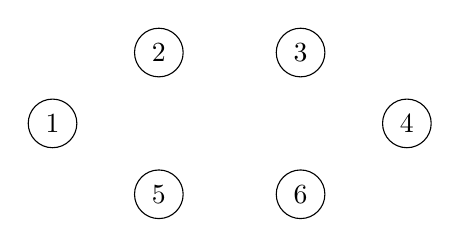
\begin{tikzpicture}[scale=0.9]
\node[draw, circle] (1) at (1.5,2) {$1$};
\node[draw, circle] (2) at (3,3) {$2$};
\node[draw, circle] (3) at (5,3) {$3$};
\node[draw, circle] (4) at (6.5,2) {$4$};
\node[draw, circle] (5) at (3,1) {$5$};
\node[draw, circle] (6) at (5,1) {$6$};
%\path[draw,thick,-] (1) -- node[font=\small,label=above:3] {} (2);
%\path[draw,thick,-] (2) -- node[font=\small,label=above:5] {} (3);
%\path[draw,thick,-] (3) -- node[font=\small,label=above:9] {} (4);
%\path[draw,thick,-] (1) -- node[font=\small,label=below:5] {} (5);
%\path[draw,thick,-] (5) -- node[font=\small,label=below:2] {} (6);
%\path[draw,thick,-] (6) -- node[font=\small,label=below:7] {} (4);
%\path[draw,thick,-] (2) -- node[font=\small,label=left:6] {} (5);
%\path[draw,thick,-] (3) -- node[font=\small,label=left:3] {} (6);
\end{tikzpicture}
\end{center}
Prvi brid koji se dodaje u stablo je
brid 5--6 koji stvara komponentu $\{5,6\}$
spajanjem komponenata $\{5\}$ i $\{6\}$:

\begin{center}
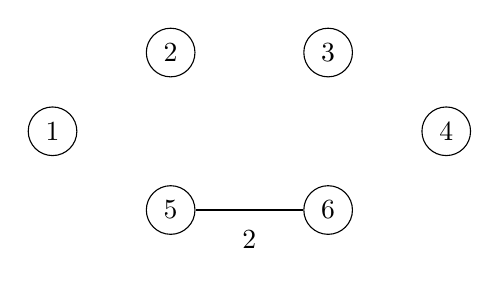
\begin{tikzpicture}
\node[draw, circle] (1) at (1.5,2) {$1$};
\node[draw, circle] (2) at (3,3) {$2$};
\node[draw, circle] (3) at (5,3) {$3$};
\node[draw, circle] (4) at (6.5,2) {$4$};
\node[draw, circle] (5) at (3,1) {$5$};
\node[draw, circle] (6) at (5,1) {$6$};

%\path[draw,thick,-] (1) -- node[font=\small,label=above:3] {} (2);
%\path[draw,thick,-] (2) -- node[font=\small,label=above:5] {} (3);
%\path[draw,thick,-] (3) -- node[font=\small,label=above:9] {} (4);
%\path[draw,thick,-] (1) -- node[font=\small,label=below:5] {} (5);
\path[draw,thick,-] (5) -- node[font=\small,label=below:2] {} (6);
%\path[draw,thick,-] (6) -- node[font=\small,label=below:7] {} (4);
%\path[draw,thick,-] (2) -- node[font=\small,label=left:6] {} (5);
%\path[draw,thick,-] (3) -- node[font=\small,label=left:3] {} (6);
\end{tikzpicture}
\end{center}
Nakon toga se na sličan način dodaju bridovi 1--2, 3--6 i 1--5:

\begin{center}
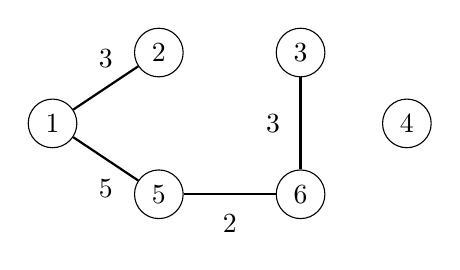
\begin{tikzpicture}[scale=0.9]
\node[draw, circle] (1) at (1.5,2) {$1$};
\node[draw, circle] (2) at (3,3) {$2$};
\node[draw, circle] (3) at (5,3) {$3$};
\node[draw, circle] (4) at (6.5,2) {$4$};
\node[draw, circle] (5) at (3,1) {$5$};
\node[draw, circle] (6) at (5,1) {$6$};

\path[draw,thick,-] (1) -- node[font=\small,label=above:3] {} (2);
%\path[draw,thick,-] (2) -- node[font=\small,label=above:5] {} (3);
%\path[draw,thick,-] (3) -- node[font=\small,label=above:9] {} (4);
\path[draw,thick,-] (1) -- node[font=\small,label=below:5] {} (5);
\path[draw,thick,-] (5) -- node[font=\small,label=below:2] {} (6);
%\path[draw,thick,-] (6) -- node[font=\small,label=below:7] {} (4);
%\path[draw,thick,-] (2) -- node[font=\small,label=left:6] {} (5);
\path[draw,thick,-] (3) -- node[font=\small,label=left:3] {} (6);
\end{tikzpicture}
\end{center}

Nakon tih koraka većina komponenata je spojena
te u stablu postoje dvije komponente:
$\{1,2,3,5,6\}$ i $\{4\}$.

Sljedeći brid u listi je brid 2--3,
no on neće biti uključen u stablo jer
su čvorovi 2 i 3 već u istoj komponenti.
Iz istog razloga brid 2--5 neće biti uključen u stablo.

\begin{samepage}
Na kraju će brid 4--6 biti uključen u stablo:

\begin{center}
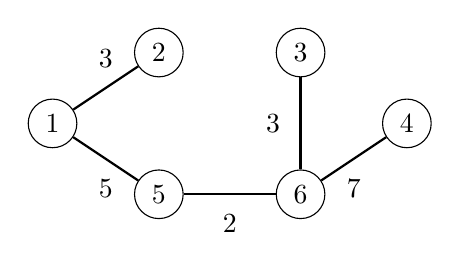
\begin{tikzpicture}[scale=0.9]
\node[draw, circle] (1) at (1.5,2) {$1$};
\node[draw, circle] (2) at (3,3) {$2$};
\node[draw, circle] (3) at (5,3) {$3$};
\node[draw, circle] (4) at (6.5,2) {$4$};
\node[draw, circle] (5) at (3,1) {$5$};
\node[draw, circle] (6) at (5,1) {$6$};

\path[draw,thick,-] (1) -- node[font=\small,label=above:3] {} (2);
%\path[draw,thick,-] (2) -- node[font=\small,label=above:5] {} (3);
%\path[draw,thick,-] (3) -- node[font=\small,label=above:9] {} (4);
\path[draw,thick,-] (1) -- node[font=\small,label=below:5] {} (5);
\path[draw,thick,-] (5) -- node[font=\small,label=below:2] {} (6);
\path[draw,thick,-] (6) -- node[font=\small,label=below:7] {} (4);
%\path[draw,thick,-] (2) -- node[font=\small,label=left:6] {} (5);
\path[draw,thick,-] (3) -- node[font=\small,label=left:3] {} (6);
\end{tikzpicture}
\end{center}
\end{samepage}

Nakon toga algoritam neće dodati nijedan
novi brid jer je graf povezan
i između svaka dva čvora postoji put.
Dobiveni graf je minimalno razapinjuće stablo
težine $2+3+3+5+7=20$.

\subsubsection{Zašto ovo funkcionira?}

Dobro je pitanje zašto Kruskalov algoritam funkcionira.
Zašto pohlepna strategija garantira da ćemo
naći minimalno razapinjuće stablo?

Pogledajmo što se dogodi ako brid najmanje težine u
grafu \emph{nije} uključen u razapinjuće stablo.
Na primjer, pretpostavimo da razapinjuće stablo
prethodnog grafa ne sadrži
brid najmanje težine 5--6.
Ne znamo točnu strukturu takvog razapinjućeg stabla,
no u svakom slučaju ono mora sadržavati neke bridove.
Pretpostavimo da bi stablo bilo sljedeće:

\begin{center}
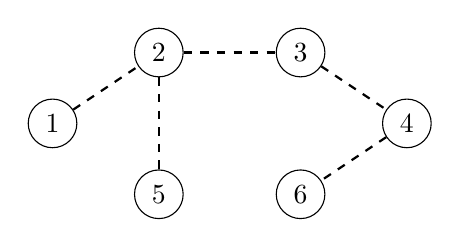
\begin{tikzpicture}[scale=0.9]
\node[draw, circle] (1) at (1.5,2) {$1$};
\node[draw, circle] (2) at (3,3) {$2$};
\node[draw, circle] (3) at (5,3) {$3$};
\node[draw, circle] (4) at (6.5,2) {$4$};
\node[draw, circle] (5) at (3,1) {$5$};
\node[draw, circle] (6) at (5,1) {$6$};

\path[draw,thick,-,dashed] (1) -- (2);
\path[draw,thick,-,dashed] (2) -- (5);
\path[draw,thick,-,dashed] (2) -- (3);
\path[draw,thick,-,dashed] (3) -- (4);
\path[draw,thick,-,dashed] (4) -- (6);
\end{tikzpicture}
\end{center}

Međutim, nije moguće da gornje stablo
bude minimalno razapinjuće stablo tog grafa.
Razlog je to što možemo ukloniti jedan brid
iz stabla i zamijeniti ga bridom najmanje težine 5--6.
To daje razapinjuće stablo čija je težina
\emph{manja}:

\begin{center}
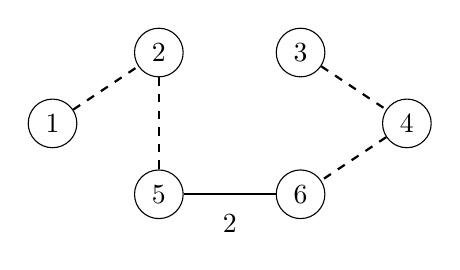
\begin{tikzpicture}[scale=0.9]
\node[draw, circle] (1) at (1.5,2) {$1$};
\node[draw, circle] (2) at (3,3) {$2$};
\node[draw, circle] (3) at (5,3) {$3$};
\node[draw, circle] (4) at (6.5,2) {$4$};
\node[draw, circle] (5) at (3,1) {$5$};
\node[draw, circle] (6) at (5,1) {$6$};

\path[draw,thick,-,dashed] (1) -- (2);
\path[draw,thick,-,dashed] (2) -- (5);
\path[draw,thick,-,dashed] (3) -- (4);
\path[draw,thick,-,dashed] (4) -- (6);
\path[draw,thick,-] (5) -- node[font=\small,label=below:2] {} (6);
\end{tikzpicture}
\end{center}

Zbog toga je uvijek optimalno
u stablo uključiti brid najmanje težine
kako bismo dobili minimalno razapinjuće stablo.
Sličnim argumentom možemo pokazati da je
također optimalno u stablo dodati sljedeći brid
po redoslijedu težina, i tako dalje.
Dakle, Kruskalov algoritam radi ispravno i
uvijek daje minimalno razapinjuće stablo.

\subsubsection{Implementacija}

Pri implementaciji Kruskalovog algoritma
prikladno je koristiti
prikaz grafa listom bridova.
Prva faza algoritma sortira
bridove u listi u $O(m \log m)$ vremenu.
Nakon toga druga faza algoritma
gradi minimalno razapinjuće stablo na sljedeći način:

\begin{lstlisting}
for (...) {
  if (!same(a,b)) unite(a,b);
}
\end{lstlisting}

Petlja prolazi kroz bridove u listi
i uvijek obrađuje brid $a$--$b$
gdje su $a$ i $b$ dva čvora.
Potrebne su dvije funkcije:
funkcija \texttt{same} određuje
jesu li $a$ i $b$ u istoj komponenti,
a funkcija \texttt{unite}
spaja komponente koje sadrže $a$ i $b$.

Problem je kako efikasno implementirati
funkcije \texttt{same} i \texttt{unite}.
Jedna je mogućnost implementirati funkciju
\texttt{same} kao obilazak grafa i provjeriti možemo li
doći od čvora $a$ do čvora $b$.
Međutim, vremenska složenost takve funkcije
bila bi $O(n+m)$
i dobiveni algoritam bio bi spor
jer će funkcija \texttt{same} biti pozvana za svaki brid u grafu.

Problem ćemo riješiti pomoću union-find strukture
koja obje funkcije implementira u $O(\log n)$ vremenu.
Stoga će vremenska složenost Kruskalovog algoritma
biti $O(m \log n)$ nakon sortiranja liste bridova.

\section{Union-find struktura}

\index{union-find struktura}

\key{Union-find struktura} održava
kolekciju skupova.
Skupovi su disjunktni, pa nijedan element
ne pripada više od jednom skupu.
Podržane su dvije operacije u $O(\log n)$ vremenu:
operacija \texttt{unite} spaja dva skupa,
a operacija \texttt{find} nalazi predstavnika
skupa koji sadrži zadani element\footnote{Strukturu prikazanu ovdje
uveli su 1971. godine J. D. Hopcroft i J. D. Ullman \cite{hop71}.
Kasnije, 1975. godine, R. E. Tarjan je proučavao sofisticiraniju varijantu
te strukture \cite{tar75} o kojoj se danas govori u mnogim
udžbenicima o algoritmima.}.

\subsubsection{Struktura}

U union-find strukturi jedan element u svakom skupu
je predstavnik tog skupa,
a od svakog drugog elementa skupa postoji lanac
do predstavnika.
Na primjer, pretpostavimo da su skupovi
$\{1,4,7\}$, $\{5\}$ i $\{2,3,6,8\}$:
\begin{center}
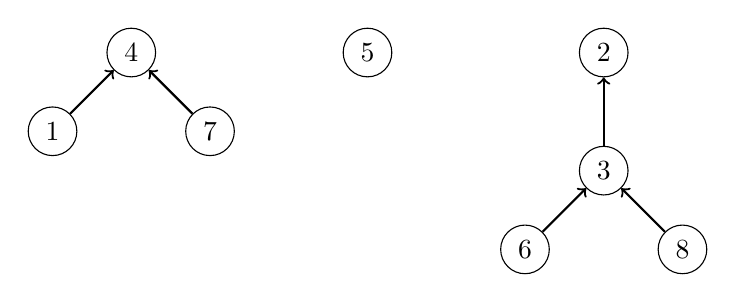
\begin{tikzpicture}
\node[draw, circle] (1) at (0,-1) {$1$};
\node[draw, circle] (2) at (7,0) {$2$};
\node[draw, circle] (3) at (7,-1.5) {$3$};
\node[draw, circle] (4) at (1,0) {$4$};
\node[draw, circle] (5) at (4,0) {$5$};
\node[draw, circle] (6) at (6,-2.5) {$6$};
\node[draw, circle] (7) at (2,-1) {$7$};
\node[draw, circle] (8) at (8,-2.5) {$8$};

\path[draw,thick,->] (1) -- (4);
\path[draw,thick,->] (7) -- (4);

\path[draw,thick,->] (3) -- (2);
\path[draw,thick,->] (6) -- (3);
\path[draw,thick,->] (8) -- (3);

\end{tikzpicture}
\end{center}
U ovom slučaju predstavnici
skupova su 4, 5 i 2.
Predstavnika bilo kojeg elementa možemo naći
slijedeći lanac koji počinje u tom elementu.
Na primjer, element 2 je predstavnik
za element 6 jer
slijedimo lanac $6 \rightarrow 3 \rightarrow 2$.
Dva elementa pripadaju istom skupu točno onda kad
su im predstavnici jednaki.

Dva skupa možemo spojiti tako da
predstavnika jednog skupa povežemo s
predstavnikom drugog skupa.
Na primjer, skupovi
$\{1,4,7\}$ i $\{2,3,6,8\}$
mogu se spojiti na sljedeći način:
\begin{center}
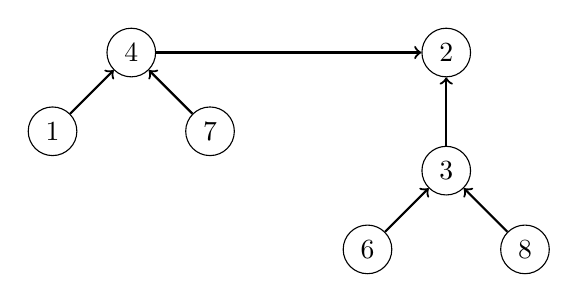
\begin{tikzpicture}
\node[draw, circle] (1) at (2,-1) {$1$};
\node[draw, circle] (2) at (7,0) {$2$};
\node[draw, circle] (3) at (7,-1.5) {$3$};
\node[draw, circle] (4) at (3,0) {$4$};
\node[draw, circle] (6) at (6,-2.5) {$6$};
\node[draw, circle] (7) at (4,-1) {$7$};
\node[draw, circle] (8) at (8,-2.5) {$8$};

\path[draw,thick,->] (1) -- (4);
\path[draw,thick,->] (7) -- (4);

\path[draw,thick,->] (3) -- (2);
\path[draw,thick,->] (6) -- (3);
\path[draw,thick,->] (8) -- (3);

\path[draw,thick,->] (4) -- (2);
\end{tikzpicture}
\end{center}

Dobiveni skup sadrži elemente
$\{1,2,3,4,6,7,8\}$.
Od sada je element 2 predstavnik
cijelog skupa, a stari predstavnik 4
pokazuje na element 2.

Efikasnost union-find strukture ovisi o tome
kako se skupovi spajaju.
Pokazuje se da možemo slijediti jednostavnu strategiju:
predstavnika \emph{manjeg} skupa uvijek
povežemo s predstavnikom \emph{većeg} skupa
(a ako su skupovi jednake veličine,
izbor može biti proizvoljan).
Uz tu strategiju dužina svakog lanca
bit će $O(\log n)$, pa predstavnika
svakog elementa možemo
efikasno naći slijedeći odgovarajući lanac.

\subsubsection{Implementacija}

Union-find strukturu možemo implementirati
pomoću nizova.
U sljedećoj implementaciji
niz \texttt{link} za svaki element sadrži
sljedeći element
u lancu ili sam taj element ako je
predstavnik,
a niz \texttt{size} za svakog predstavnika označava
veličinu odgovarajućeg skupa.

Na početku svaki element pripada zasebnom skupu:
\begin{lstlisting}
for (int i = 1; i <= n; i++) link[i] = i;
for (int i = 1; i <= n; i++) size[i] = 1;
\end{lstlisting}

Funkcija \texttt{find} vraća
predstavnika elementa $x$.
Predstavnika možemo naći slijedeći
lanac koji počinje u $x$.

\begin{lstlisting}
int find(int x) {
    while (x != link[x]) x = link[x];
    return x;
}
\end{lstlisting}

Funkcija \texttt{same} provjerava
pripadaju li elementi $a$ i $b$ istom skupu.
To se lako može učiniti koristeći
funkciju \texttt{find}:

\begin{lstlisting}
bool same(int a, int b) {
    return find(a) == find(b);
}
\end{lstlisting}

\begin{samepage}
Funkcija \texttt{unite} spaja skupove
koji sadrže elemente $a$ i $b$
(elementi moraju biti u različitim skupovima).
Funkcija najprije nalazi predstavnike
skupova, a zatim povezuje manji
skup s većim skupom.

\begin{lstlisting}
void unite(int a, int b) {
    a = find(a);
    b = find(b);
    if (size[a] < size[b]) swap(a,b);
    size[a] += size[b];
    link[b] = a;
}
\end{lstlisting}
\end{samepage}

Vremenska složenost funkcije \texttt{find}
je $O(\log n)$ pod pretpostavkom da je dužina svakog
lanca $O(\log n)$.
U tom slučaju funkcije \texttt{same} i \texttt{unite}
također rade u $O(\log n)$ vremenu.
Funkcija \texttt{unite} osigurava da je
dužina svakog lanca $O(\log n)$ time što
manji skup povezuje s većim skupom.

\section{Primov algoritam}

\index{Primov algoritam}

\key{Primov algoritam}\footnote{Algoritam je
nazvan po R. C. Primu koji ga je objavio 1957. godine \cite{pri57}.
Međutim, isti je algoritam još 1930. godine otkrio
V. Jarník.} alternativna je metoda
za traženje minimalnog razapinjućeg stabla.
Algoritam najprije dodaje proizvoljan čvor
u stablo.
Nakon toga algoritam uvijek odabire
brid najmanje težine koji
u stablo dodaje novi čvor.
Na kraju su svi čvorovi dodani u stablo
i minimalno razapinjuće stablo je nađeno.

Primov algoritam sličan je Dijkstrinom algoritmu.
Razlika je u tome što Dijkstrin algoritam uvijek
odabire brid čija je udaljenost od početnog
čvora najmanja, dok Primov algoritam jednostavno odabire
brid najmanje težine koji u stablo dodaje novi čvor.

\subsubsection{Primjer}

Razmotrimo kako Primov algoritam radi
na sljedećem grafu:

\begin{center}
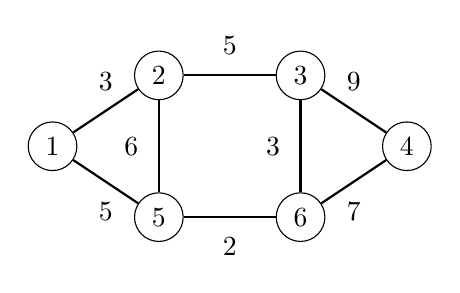
\begin{tikzpicture}[scale=0.9]
\node[draw, circle] (1) at (1.5,2) {$1$};
\node[draw, circle] (2) at (3,3) {$2$};
\node[draw, circle] (3) at (5,3) {$3$};
\node[draw, circle] (4) at (6.5,2) {$4$};
\node[draw, circle] (5) at (3,1) {$5$};
\node[draw, circle] (6) at (5,1) {$6$};
\path[draw,thick,-] (1) -- node[font=\small,label=above:3] {} (2);
\path[draw,thick,-] (2) -- node[font=\small,label=above:5] {} (3);
\path[draw,thick,-] (3) -- node[font=\small,label=above:9] {} (4);
\path[draw,thick,-] (1) -- node[font=\small,label=below:5] {} (5);
\path[draw,thick,-] (5) -- node[font=\small,label=below:2] {} (6);
\path[draw,thick,-] (6) -- node[font=\small,label=below:7] {} (4);
\path[draw,thick,-] (2) -- node[font=\small,label=left:6] {} (5);
\path[draw,thick,-] (3) -- node[font=\small,label=left:3] {} (6);

%\path[draw=red,thick,-,line width=2pt] (5) -- (6);
\end{tikzpicture}
\end{center}
Na početku nema bridova između čvorova:
\begin{center}
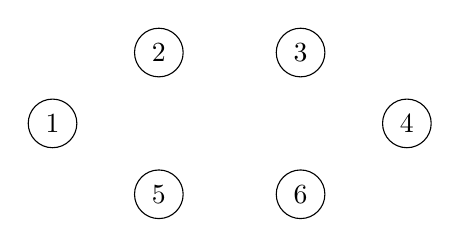
\begin{tikzpicture}[scale=0.9]
\node[draw, circle] (1) at (1.5,2) {$1$};
\node[draw, circle] (2) at (3,3) {$2$};
\node[draw, circle] (3) at (5,3) {$3$};
\node[draw, circle] (4) at (6.5,2) {$4$};
\node[draw, circle] (5) at (3,1) {$5$};
\node[draw, circle] (6) at (5,1) {$6$};
%\path[draw,thick,-] (1) -- node[font=\small,label=above:3] {} (2);
%\path[draw,thick,-] (2) -- node[font=\small,label=above:5] {} (3);
%\path[draw,thick,-] (3) -- node[font=\small,label=above:9] {} (4);
%\path[draw,thick,-] (1) -- node[font=\small,label=below:5] {} (5);
%\path[draw,thick,-] (5) -- node[font=\small,label=below:2] {} (6);
%\path[draw,thick,-] (6) -- node[font=\small,label=below:7] {} (4);
%\path[draw,thick,-] (2) -- node[font=\small,label=left:6] {} (5);
%\path[draw,thick,-] (3) -- node[font=\small,label=left:3] {} (6);
\end{tikzpicture}
\end{center}
Početni čvor može biti proizvoljan,
pa odaberimo čvor 1.
Najprije dodajemo čvor 2 koji je spojen
bridom težine 3:
\begin{center}
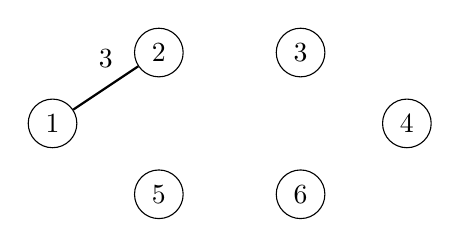
\begin{tikzpicture}[scale=0.9]
\node[draw, circle] (1) at (1.5,2) {$1$};
\node[draw, circle] (2) at (3,3) {$2$};
\node[draw, circle] (3) at (5,3) {$3$};
\node[draw, circle] (4) at (6.5,2) {$4$};
\node[draw, circle] (5) at (3,1) {$5$};
\node[draw, circle] (6) at (5,1) {$6$};
\path[draw,thick,-] (1) -- node[font=\small,label=above:3] {} (2);
%\path[draw,thick,-] (2) -- node[font=\small,label=above:5] {} (3);
%\path[draw,thick,-] (3) -- node[font=\small,label=above:9] {} (4);
%\path[draw,thick,-] (1) -- node[font=\small,label=below:5] {} (5);
%\path[draw,thick,-] (5) -- node[font=\small,label=below:2] {} (6);
%\path[draw,thick,-] (6) -- node[font=\small,label=below:7] {} (4);
%\path[draw,thick,-] (2) -- node[font=\small,label=left:6] {} (5);
%\path[draw,thick,-] (3) -- node[font=\small,label=left:3] {} (6);
\end{tikzpicture}
\end{center}

Nakon toga postoje dva brida težine 5,
pa u stablo možemo dodati čvor 3 ili čvor 5.
Dodajmo najprije čvor 3:
\begin{center}
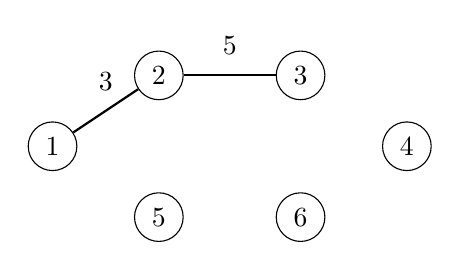
\begin{tikzpicture}[scale=0.9]
\node[draw, circle] (1) at (1.5,2) {$1$};
\node[draw, circle] (2) at (3,3) {$2$};
\node[draw, circle] (3) at (5,3) {$3$};
\node[draw, circle] (4) at (6.5,2) {$4$};
\node[draw, circle] (5) at (3,1) {$5$};
\node[draw, circle] (6) at (5,1) {$6$};
\path[draw,thick,-] (1) -- node[font=\small,label=above:3] {} (2);
\path[draw,thick,-] (2) -- node[font=\small,label=above:5] {} (3);
%\path[draw,thick,-] (3) -- node[font=\small,label=above:9] {} (4);
%\path[draw,thick,-] (1) -- node[font=\small,label=below:5] {} (5);
%\path[draw,thick,-] (5) -- node[font=\small,label=below:2] {} (6);
%\path[draw,thick,-] (6) -- node[font=\small,label=below:7] {} (4);
%\path[draw,thick,-] (2) -- node[font=\small,label=left:6] {} (5);
%\path[draw,thick,-] (3) -- node[font=\small,label=left:3] {} (6);
\end{tikzpicture}
\end{center}

\begin{samepage}
Postupak se nastavlja dok svi čvorovi ne budu uključeni u stablo:
\begin{center}
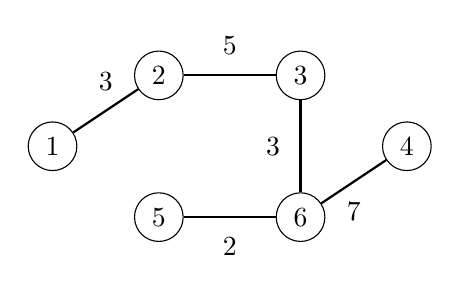
\begin{tikzpicture}[scale=0.9]
\node[draw, circle] (1) at (1.5,2) {$1$};
\node[draw, circle] (2) at (3,3) {$2$};
\node[draw, circle] (3) at (5,3) {$3$};
\node[draw, circle] (4) at (6.5,2) {$4$};
\node[draw, circle] (5) at (3,1) {$5$};
\node[draw, circle] (6) at (5,1) {$6$};
\path[draw,thick,-] (1) -- node[font=\small,label=above:3] {} (2);
\path[draw,thick,-] (2) -- node[font=\small,label=above:5] {} (3);
%\path[draw,thick,-] (3) -- node[font=\small,label=above:9] {} (4);
%\path[draw,thick,-] (1) -- node[font=\small,label=below:5] {} (5);
\path[draw,thick,-] (5) -- node[font=\small,label=below:2] {} (6);
\path[draw,thick,-] (6) -- node[font=\small,label=below:7] {} (4);
%\path[draw,thick,-] (2) -- node[font=\small,label=left:6] {} (5);
\path[draw,thick,-] (3) -- node[font=\small,label=left:3] {} (6);
\end{tikzpicture}
\end{center}
\end{samepage}

\subsubsection{Implementacija}

Kao i Dijkstrin algoritam, Primov algoritam možemo
efikasno implementirati pomoću prioritetnog reda.
Prioritetni red trebao bi sadržavati sve čvorove
koji se mogu spojiti s trenutnom komponentom pomoću
jednog brida, u rastućem redoslijedu težina
odgovarajućih bridova.

Vremenska složenost Primovog algoritma je
$O(n + m \log m)$, što je jednako vremenskoj složenosti
Dijkstrinog algoritma.
U praksi su i Primov i Kruskalov algoritam
efikasni, a izbor algoritma
stvar je ukusa.
Ipak, većina natjecatelja u programiranju koristi Kruskalov algoritam.